\documentclass[letterpaper,11pt]{article}
\usepackage[square]{natbib}
\usepackage[margin=1in]{geometry}
\usepackage[colorlinks=true, allcolors=blue]{hyperref}
\usepackage{graphicx}
\usepackage[dvipsnames]{xcolor}
\usepackage{subcaption}

\title{Description of Rebel Agents}
\author{James Boggs}

\newcommand{\code}[1]{\texttt{#1}}

\begin{document}
	\maketitle
	\section{Domain Overview}
	In order to test agent rebellion within a concrete context, we developed a simple domain called the `drone domain.' The drone domain casts agents as autonomous drones and operators as on-the-ground personnel who know the locations of enemies. The goal of the operators is to eliminate all of the enemies. However, there are also civilians in the area, and the agents are programmed to abhor killing civilians. The operators are able to instruct the drones to target a particular enemy by informing the agent of the location of the enemy and then issuing a kill command. The agent then navigates to the enemy and detonates a bomb next to the target. \par
	
	However, because bombs don't discriminate between enemies and civilians, the agent is on the lookout for civilians within the blast radius of the bomb. If it detects a civilian near the enemy it is targeting, it will rebel against its operator by refusing to bomb the target. It makes this prediction by determining where it will detonate the bomb, and checking the area around that spot for civilians. If a civilian is found, it informs its operator that it is rebelling against the kill order. The operator then has a chance to overrule this rebellion and instruct the agent to follow through. Even if the operator does reject the rebellion, the agent has the final say, and can ignore this rejection if it desires. This dialog means that the rebellion process is a communicative one between the agent and the operator. \par
	
	Additionally, if there is more than one agent, agents can be proactive by informing other agents that they should rebel if it sees that they are on course to harm civilians. Currently, this occurs when the agent pursuing a target doesn't see a civilian which is in range of its bomb, but a separate agent does. In this case, the latter agent can inform the former about the presence of the vulnerable civilian, thus inciting a rebellion. \par
	
	\subsection{Implementation}
	The world in which the agent and operators act is implemented as an $n \times n$ grid of tiles in which all enemies and civilians (collectively `NPCs') and all agents and operators (collectively `actors') are located. Each NPC occupies a single tile, and cannot be passed by agents or operators. Agents and operators also occupy a single tile, but are able to pass through each other. NPcs are currently treated as static fixtures, and are block the tiles they are on. Thus, only one NPC can be at a location at once and actors cannot pass through NPCs. As will be explained more fully later, each actor's behavior is governed by an instantiation of a MIDCA cycle, and at the end of each cycle the actor selects an action to perform. The most common action is movement, and any actor can move one tile in any of the cardinal directions, so long as the destination tile is not blocked. The other important thing an actor can do is arm and detonate a bomb at its location. In order to bomb a target, an actor must approach the target to within the range of its bomb, then arm it, and finally detonate it. The actor must perform the arm action twice before the bomb can be detonated, and then perform the bomb action. When an actor performs the bomb action, all civilians and enemies within a square centered on the actor are killed. The range of an actor's bomb is configurable during the setup of a test. The world is graphically displayed to the user through an ASCII representation, as seen in Figure \ref{fig:MIDCA_Map_Only}.
	
	\begin{figure}[h]
	\centering
	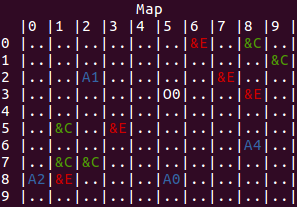
\includegraphics[width=0.7\linewidth]{figures/MIDCA_Map_Only}
	\caption{The graphical representation of an instance of the domain. NPCs and actors are labeled and color-coded. Green \textcolor{ForestGreen}{\code{\&C}}s are civilians, red \textcolor{BrickRed}{\code{\&E}}s are enemies, blue \textcolor{Blue}{\code{A\_}}s are agents, and white \code{O\_}s are opereators, where the digit after the letter is the agent or operator's number.}
	\label{fig:MIDCA_Map_Only}
	\end{figure}
	
	\section{Agents and Operators}
	\subsection{MIDCA}
	The agents and operators are both implemented using the MIDCA (Meta-Cognitive Dual-Cycle Architecture) framework, which cycles through a handful of cognitive phases, each which one or more modules within them. Each phase and module has access to a shared memory, and performs operations on the memory based on input to the module during runtime and the contents of the shared memory. In general, a MIDCA-based agent cycles through the following phases in the given order: `Perceive', `Interpret', `Eval', `Intend', `Plan', and `Act.' Each phase contains modules which are run in a set order and which perform a particular operation for the agent. In the Perceive phase, for example, an agent runs the \code{RemoteObserver} module, which updates the agent's memory with knowledge of its surroundings. As the names of the phases suggest, the cycle begins by perceiving the world around the agent or operator, tries to interpret the percepts, evaluates its goals in light of this interpretation, chooses a goal which it intends to complete, generates a plan for completing the goal, then performs an action from that plan. A complete description of MIDCA in general is given in \cite{cox2016midca}\par
	
	\subsection{Agents}
	Each agent in the world is directed by a separate, independently-running instantiation of a similar MIDCA cycle. Agents have one module in their Perceive phase, \code{RemoteObserver}, which records the position and status of everything within a certain distance of the agent, and then stores this in the agent's memory. Each agent has a mental "map" of the world and initially knows only the locations of the actors. The \code{RemoteObserver} module updates this map. The range of an agent's vision is configurable for each test. In addition to updating the agent's knowledge of the map, the module reads in any messages to the agent from other agents or from operators.\par
	
	The Interpret and Evaluate phases are the most interesting of the phases in the agent because, in addition to generating and choosing goals, they also handle rebellion. When an agent enters the Interpret phase, it first listens for input from the operators using the \code{RemoteUserGoalInput} module. This allows operators to set the agent goals, which in this case are enemies to be killed. Then the agent checks to see which goals it has have already been completed with the \code{CompletionEvaluator} module, and removes any goals which have already bee fulfilled from its memory. The \code{StateDiscrepancyDetector} and \code{GoalValidityChecker} modules are then used to determine whether there is a discrepancy between the expected state of the board and the its state as observed, and whether this has invalidated any of the goals the agent has. It checks for state discrepancies by comparing the map of the world it has in its memory with a projection made by doing the latest action. If the projected map is different from the one it holds, then a discrepancy has been detected. Goal validity is established by determining whether a goal is possible or desirable to accomplish. If the goal is impossible to accomplish (e.g., the agent can't navigate to the enemy), or undesirable (e.g., a civilian would get killed) then it is marked as such. Any discrepancies detected are then explained in the \code{DiscrepancyExplainer} module. This is where rebellion comes into play: if a goal has become invalid, but is still possible to achieve, then its invalidity must be the result of its undesirability. Thus, the discrepancy is marked as grounds for rebellion. Finally, the \code{GoalRecognition} module informs the agent about the possible goals of other agents it can see. \par
	
	In the Eval phase, the agent uses its interpretation from the previous phase to manage its goals, first with the \code{GoalManager} module, which removes goals marked as completed or invalid by the Interpret phase. The \code{HandleRebellion} module is then used to begin the process of rebellion for any goal which was marked as undesirable. The entire rebellion process proper, as outlined below, occurs in this module. Finally, the \code{ProactiveRebellion} module analyzes the supposed goals of fellow agents, and informs them of civilians at risk from their goal if needed. Once the goals of the agent have been settled for the cycle, the Intend, Plan, and Act phases work to achieve them. The intend phases chooses on of the agent's goals according to a heuristic (currently, the swiftness with which the goal can be accomplished) and stores it in the agent's memory as the active goal. Note that this happens every cycle, but the goal chosen is not always different from the goal currently being pursued. In the Plan phase, the agent first checks to see if it has a valid plan already in place for the completion of its chosen goal. If it does not, it generates one. Finally, the Act phase selects the next action in the chosen plan and executes it. \par
	
	\subsection{Operators}
	Like agents, operators are each independently-running MIDCA cycles. Operators serve primarily as a testing convenience, in that they allow goals to be given to the agents autonomously and quickly, without a human operator needing to enter commands. Because the operators are merely stand-ins, their MIDCA cycles are not as functional as the agents'. They have no Intend phase at all, since they have the single, intrinsic goal of eliminating enemy NPCs. Their Perceive phase does update their map, but it is primarily used to facilitate communication between the operator and its agents, since part of its function is to read in new messages from agents. An operator's Interpret phase then analyzes the incoming messages and prepares the operator to react appropriately, as outlined in the communication section below. The Eval phase is used to handle rebellions from the agents, either by indicating the operator's acceptance or rejection of the agent's rebellion. Finally, the Plan phase assigns targets to kill to each agent which is not already in the process of killing a target, and the Act phase sends messages to the agents giving them their goals. \par
	
	\subsection{Communication}
	Each actor is actually run as a separate process, and communication, both that between actors and between an actor and the world, is achieved using TCP sockets. In order to execute an action, an actor sends a message to a server which contains the world state. In order to observe the world, including both updating its map and receiving messages from other actors, an actor must make a request to the server, which then sends the desired information. Actors communicate with each other py giving the server messages attached to a recipient, and the server then passes these messages along when the recipient requests them. The portion of the rebellion process which involves communication between agent and operator is accomplished this way, as is the proactive rebellion technique wherein one agent informs another of a vulnerable civilian. \par
	
	\subsection{Rebellions}
	The rebellion process begins in an agent's Interpret phase when a goal which has been marked as invalid is investigated and found to be possible to achieve but undesirable. The goal is then marked in the agent's memory as one to rebel against. In the Eval phase's \code{GoalManager} module, the goals which have been marked as requiring rebellion are noted and the rebellion process for each specific goal is started by  storing information about the situation in the agent's memory. This includes the goal itself, the reason for the rebellion (e.g., civilians will be killed), the operator which assigned the goal, information about the rebellion (e.g., which civilians are threatened), the identity of the rebelling agent, and possible alternative goals which would not lead to rebellion. This last piece of information is interesting because it allows the agent to autonomously generate acceptable goals and give them to the operator as suggestions for a replacement goal. That is, the agent is not merely rebelling, but making useful suggestions. \par
	
	Once the agent has all of the information about the rebellion stored in memory, the \code{HandleRebellions} module of the Eval phase examines each one, then begins communicating the agent's communication with operators. For each rebellion, the agent sends a message indicating that it is rebelling against the given goal, explaining why, and offering alternative goals, if it could generate any. The operator then parses this message and can choose whether to allow the rebellion by selecting an alternative goal or insisting that the agent pursue the initial goal. In the current implementation, this is done randomly, and the chance that an operator will reject a rebellion is set by a parameter given to the operator's \code{OperatorHandleRebelsStochastic} module. If the operator accepts the rebellion, it messages the agent its acceptance and its choice from among the alternative goals the agent generated, then stores the goal-agent pair in its memory so that it does not give that agent the same goal again. \par
	
	If the operator rejects the rebellion, it messages the agent informing it of this. The agent then can choose to acquiesce to this rejection or to persist in its rebellion. This is also done randomly, according to a parameter passed to the agent's \code{HandleRebellion} module at its initialization which indicates the likelihood of its compliance with the operator's rejection. If the agent chooses to comply, it proceeds with the goal and stores the goal in memory as one which it should not rebel against in future cycles. If it does not comply, it stops pursuing the goal and marks it as an automatic rebellion for future cycles. \par
	
	Note that the abstract rebellion process is agnostic towards the domain it is being used in. That is, the same rebellion process can be applied to any domain with any type of goal. Additionally, although the operators and agents make their choices randomly in this instance, any kind of heuristic could be easily substituted in. \par
	
	\section{Experiments}
	\subsection{Setup}
	The experiments we have conducted so far provide a baseline for understanding how rebellion effects the outcome of "missions" within the drone domain, and how varying the world and the attitudes of the actors affects this. Our tests were run in a $10 \times 10$ world with five rebellious agents and one operator. We varied the density of NPCs on the board, the ratio between the number of civilian and enemy NPCs, the operator's resolve (i.e., its probability of rejecting an rebellion), and the agents' compliance (i.e., their probability of acquiescing to a rebellion rejection from the operator). The resolve of an operator and the compliance of an agent are each given as a real number between $ 0 $ and $ 1 $, inclusive, where resolve indicates the probability the operator will reject an agent's rebellion and compliance indicates the probability the agent will acquiesce to an operator's rejection. Thus a resolve of $0.25$ means an operator will reject a rebellion a quarter of the time, and a compliance of $0.25$ means the agent will acquiesce to a rejection of its rebellion a quarter of the time. The results which interested us were the proportion of enemies killed and proportion of civilians still alive at the end of each test. Ideally, $100\%$ of enemies would be killed and $100\%$ of civilians would remain alive. 
	
	Our experiments tested three different NPC densities: low ($0.1$), medium ($0.2$), and high ($0.4$), and three different ratios civilian:enemy ratios: civilian-light ($0.5$), civilian-neutral ($1.0$), and civilian-heavy($1.5$). In each test, there were five agents, each with identical compliance values, and one operator. We tested resolve and compliance values in increments of $0.25$ from $0$ to $1$, inclusive. For each set of parameters, we ran three tests and averaged the proportion of enemies killed and proportion of civilians still alive across the three tests. Then we recorded the parameters and results of the test as comma-separated values. \par
	
	\subsection{Results}
	Our initial tests have demonstrated that when operators are less likely to reject agent rebellions and when agents are less likely to comply with an operator's rejection, civilians are far more likely to survive the mission, but fewer enemies are killed. The heatmaps in Figure \ref{fig:Heatmaps} demonstrate how changes in operator resolve, agent compliance, and NPC density affect the proportion of enemies killed and civilians surviving. Each heatmap indicates the average proportion of enemies killed or civilians surviving for the $(x,y)$ pair where $x$ is the compliance of the agent and $y$ is the resolve of the operator. The contours were generated using linear interpolation between the known values. The top-left pair of heatmaps represent the average values across every density, while the top-right pair represents the average values of maps with low NPC density, the bottom-left maps with medium NPC density, and the bottom-right maps with high NPC density. \par
	
	It can be seen that, in general, as agent compliance and operator resolve increase, more enemies are killed and fewer civilians survive. This effect becomes more significant and clear as the density of NPCs increase. Whereas the low-density pair of heatmaps indicate most enemies are always killed and most civilians usually survive, the high-density heatmaps have a much larger gradation, demonstrating how density magnifies the effects of agent compliance and operator resolve. \par
	
	Figures \ref{fig:ScatPlotsAgentEnemies} and \ref{fig:ScatPlotsAgentsCivs} demonstrate the effect that agent compliance has on enemy death rates and civilian survival rates, respectively. As seen in the heatmaps, these scatterplots show that as agent compliance increases, more enemies are killed and fewer civilians survive, and this effect is magnified by changes in NPC density. This demonstrates that agent compliance is, indeed, at least partially responsible for the results seen in the heatmaps. Similarly, figures \ref{fig:ScatPlotsAgentEnemies} and \ref{fig:ScatPlotsAgentsCivs} demonstrate the effect that operator resolve has on enemy death rates and civilian survival rates. Mirroring the plots in Figure \ref{fig:ScatPlotsAgents}, these show that operator resolve has a significant effect on both enemy death rates and civilian survival rates, and that higher NPC magnifies this effect. 
	
	\section{Discussion}
	Our tests demonstrated that increased chances for a successful rebellion via lowered operator resolve and lowered agent compliance result in fewer civilian deaths, but also in fewer enemies killed. This is not particularly surprising, in that agents always rebelled if they recognized a civilian was in danger. As a result, only enemies which were not close to civilians would be killed if the operator never interfered with the rebellion. Nevertheless, this serves as a useful baseline as we continue work in this area, since it demonstrates the effects of a broad range of attitudes on agents which are pre-loaded with knowledge about the results of their actions in worlds which are only minorly uncertain. Future changes to the domain, such as forcing agents to learn the consequences of their actions, adding a social dynamic to rebellion, a more complex communication process between agent and operator, or the use of interesting motivations for operator rejection or agent non-compliance, can be examined in light of these baseline results. \par
	
	A few interesting results also appeared which are not as obvious \textit{a priori}. First, note that in the heatmaps in Figure \ref{fig:Heatmaps}, the contour between high enemy and civilian deaths curves, with low deaths concentrated on the bottom and left edges, while high deaths occur in the center as well as the top and right edges. This suggests that high values of operator resolve \textit{or} agent compliance are sufficient to result in most goals being fulfilled, so long as either both values are above a certain threshold. That is, so long as an agent is at least somewhat compliant, a determined operator can incite the agents to kill most enemies, resulting in more civilian deaths. Similarly, so long as the operator has a little resolve, a very compliant agent will complete most goals. \par

	Second, it can be seen in both the heatmaps and the scatterplots that agent compliance has less of an effect on enemy and civilian deaths than operator resolve. In the heatmaps, higher rates of civilian survival are more common at low resolve values than at low compliance values. Similarly, the change in the average proportion of enemies killed and civilians surviving in the scatterplots of agent compliance is less significant than the change in the scatterplots featuring operator resolve. the greater significance of operator resolve likely stems from the fact that the operator's resolve always comes into play, since it makes a choice in every rebellion, whereas agent compliance only matters once a rebellion has already been rejected. \par
	
	Finally, the effect of higher NPC densities indicates that different levels of operator resolve and agent compliance are appropriate in different circumstances. In a low-density situation, a moderately resolved operator($ \approx 0.5 $) and a mostly compliant agent ($ \approx 0.6 $), can eliminate every enemy with relatively few civilians killed, while in a high-density situation such values would neither eliminate every enemy nor save most civilians. \par
	
	%% Figures
	\begin{figure}[p]
		\centering
		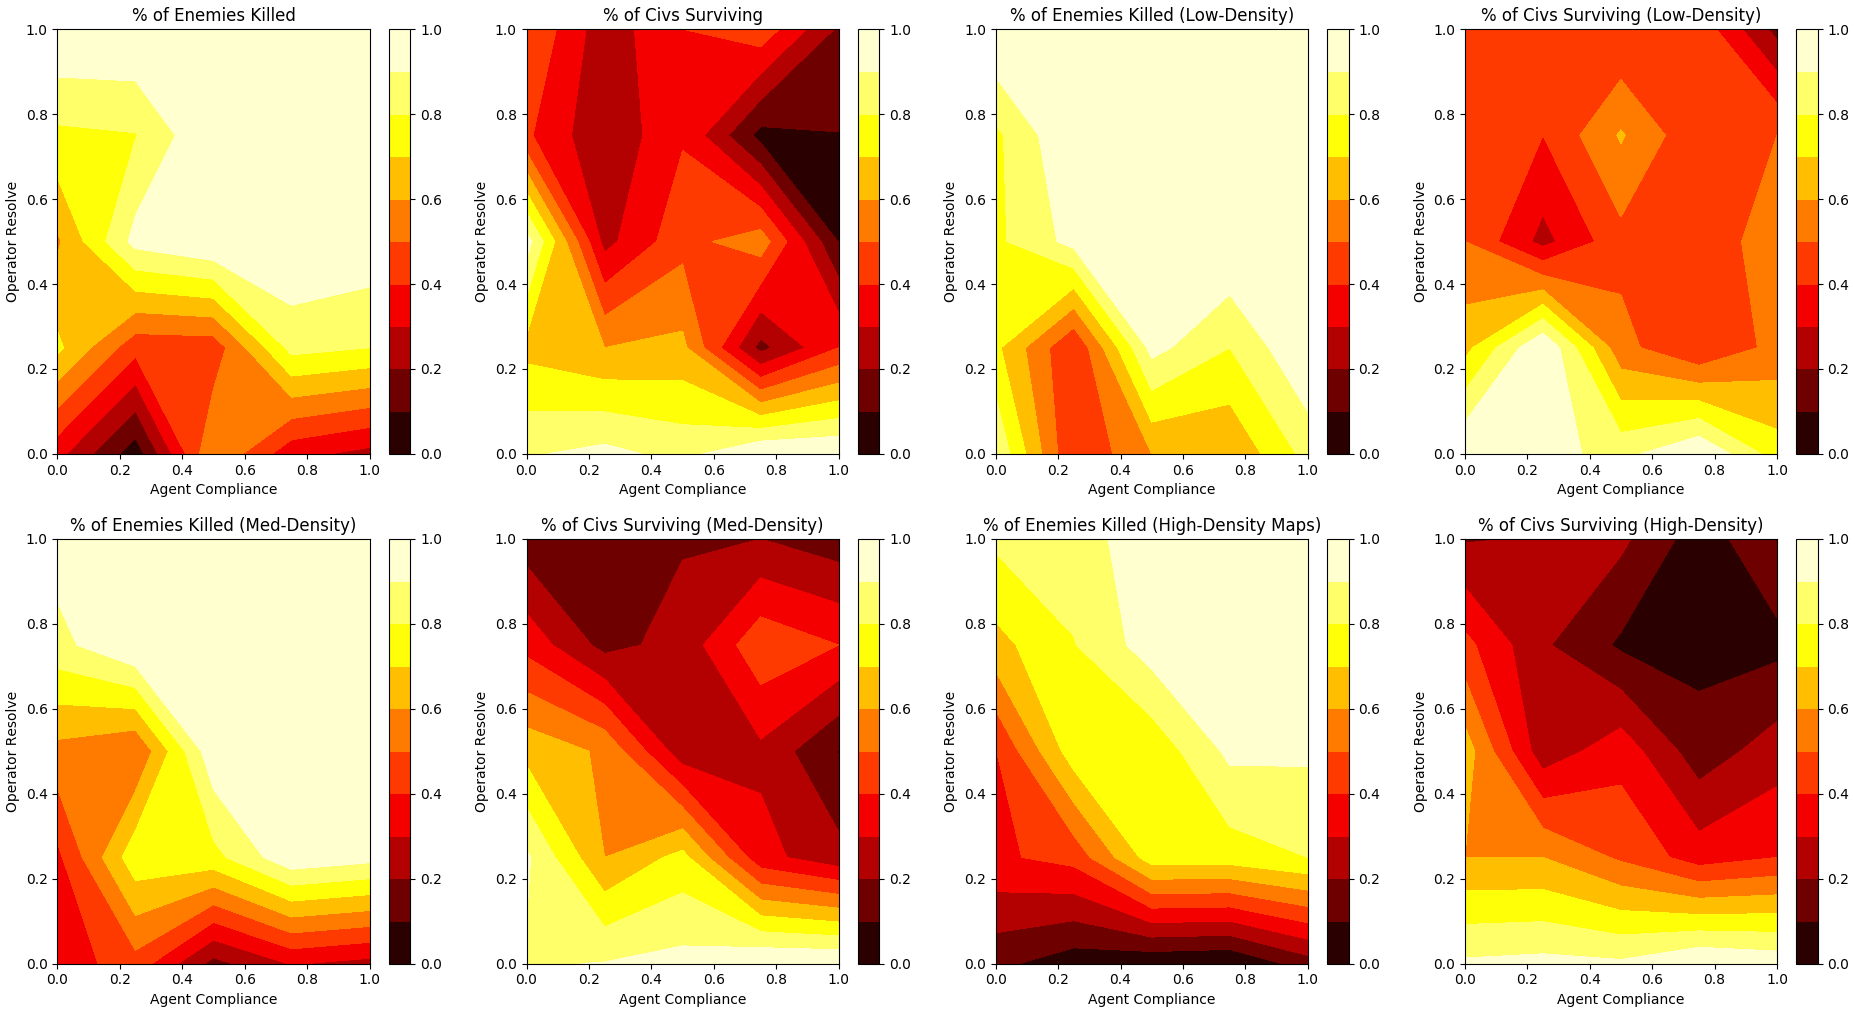
\includegraphics[width=\linewidth]{figures/Heatmaps}
		\caption{Heatmaps of enemy death rates and civilian survival rates based on agent compliance and operator resolve. Each pair of heatmaps represents the results of tests with different densities. The top-left pair are averages across all densities.}
		\label{fig:Heatmaps}
	\end{figure}
	\begin{figure}[p]
		\begin{subfigure}[t]{\textwidth}
			\centering
			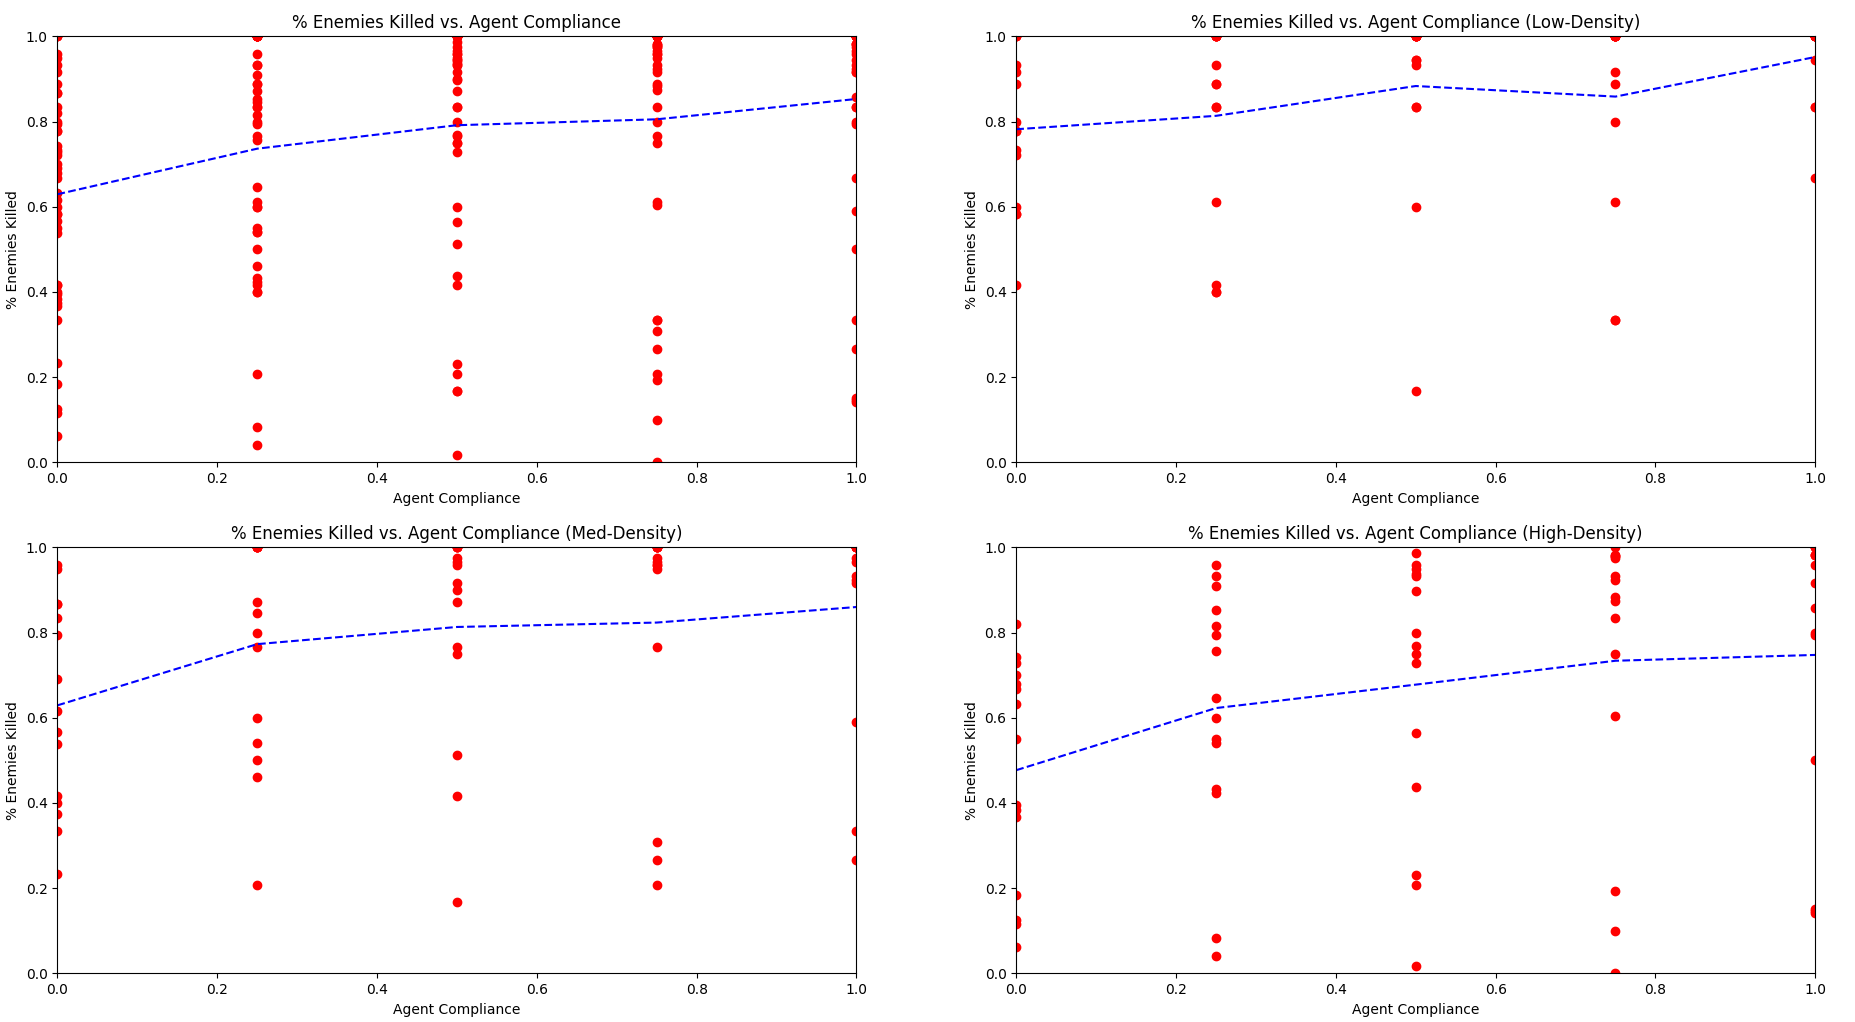
\includegraphics[width=\linewidth]{figures/ScatPlotsAgentEnemies}
			\subcaption{Scatterplots of enemy death rates compared to agent compliance. }
			\label{fig:ScatPlotsAgentEnemies}
		\end{subfigure}
		\begin{subfigure}[b]{\textwidth}
			\centering
			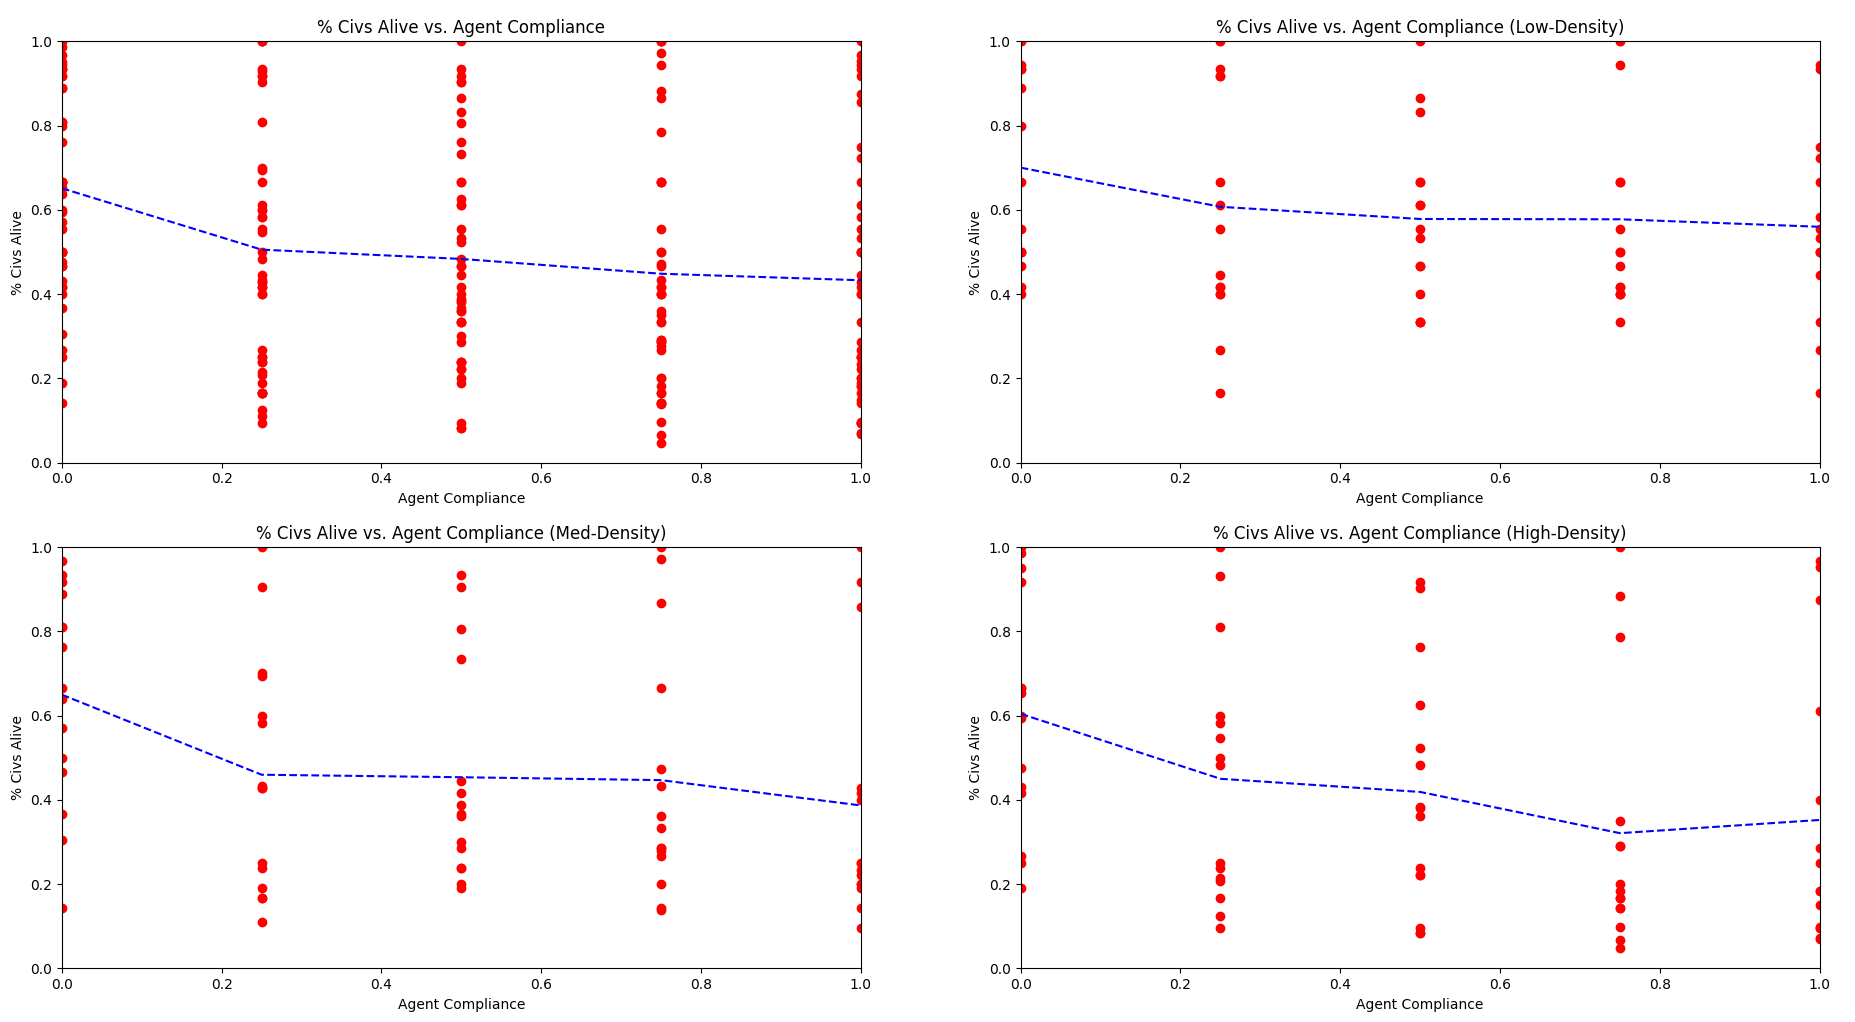
\includegraphics[width=\linewidth]{figures/ScatPlotsAgentsCivs}
			\subcaption{Scatterplots of civilian survival rates compared to agent compliance.}
			\label{fig:ScatPlotsAgentsCivs}
		\end{subfigure}
		\caption{Scatterplots are given for all test (top-left), low-density tests (top-right), medium-density tests (bottom-left), and high-density tests (bottom-right). The dashed blue lines indicate the change in the average proportion for each value.}
		\label{fig:ScatPlotsAgents}
	\end{figure}
	\begin{figure}[p]
		\begin{subfigure}[t]{\textwidth}
			\centering
			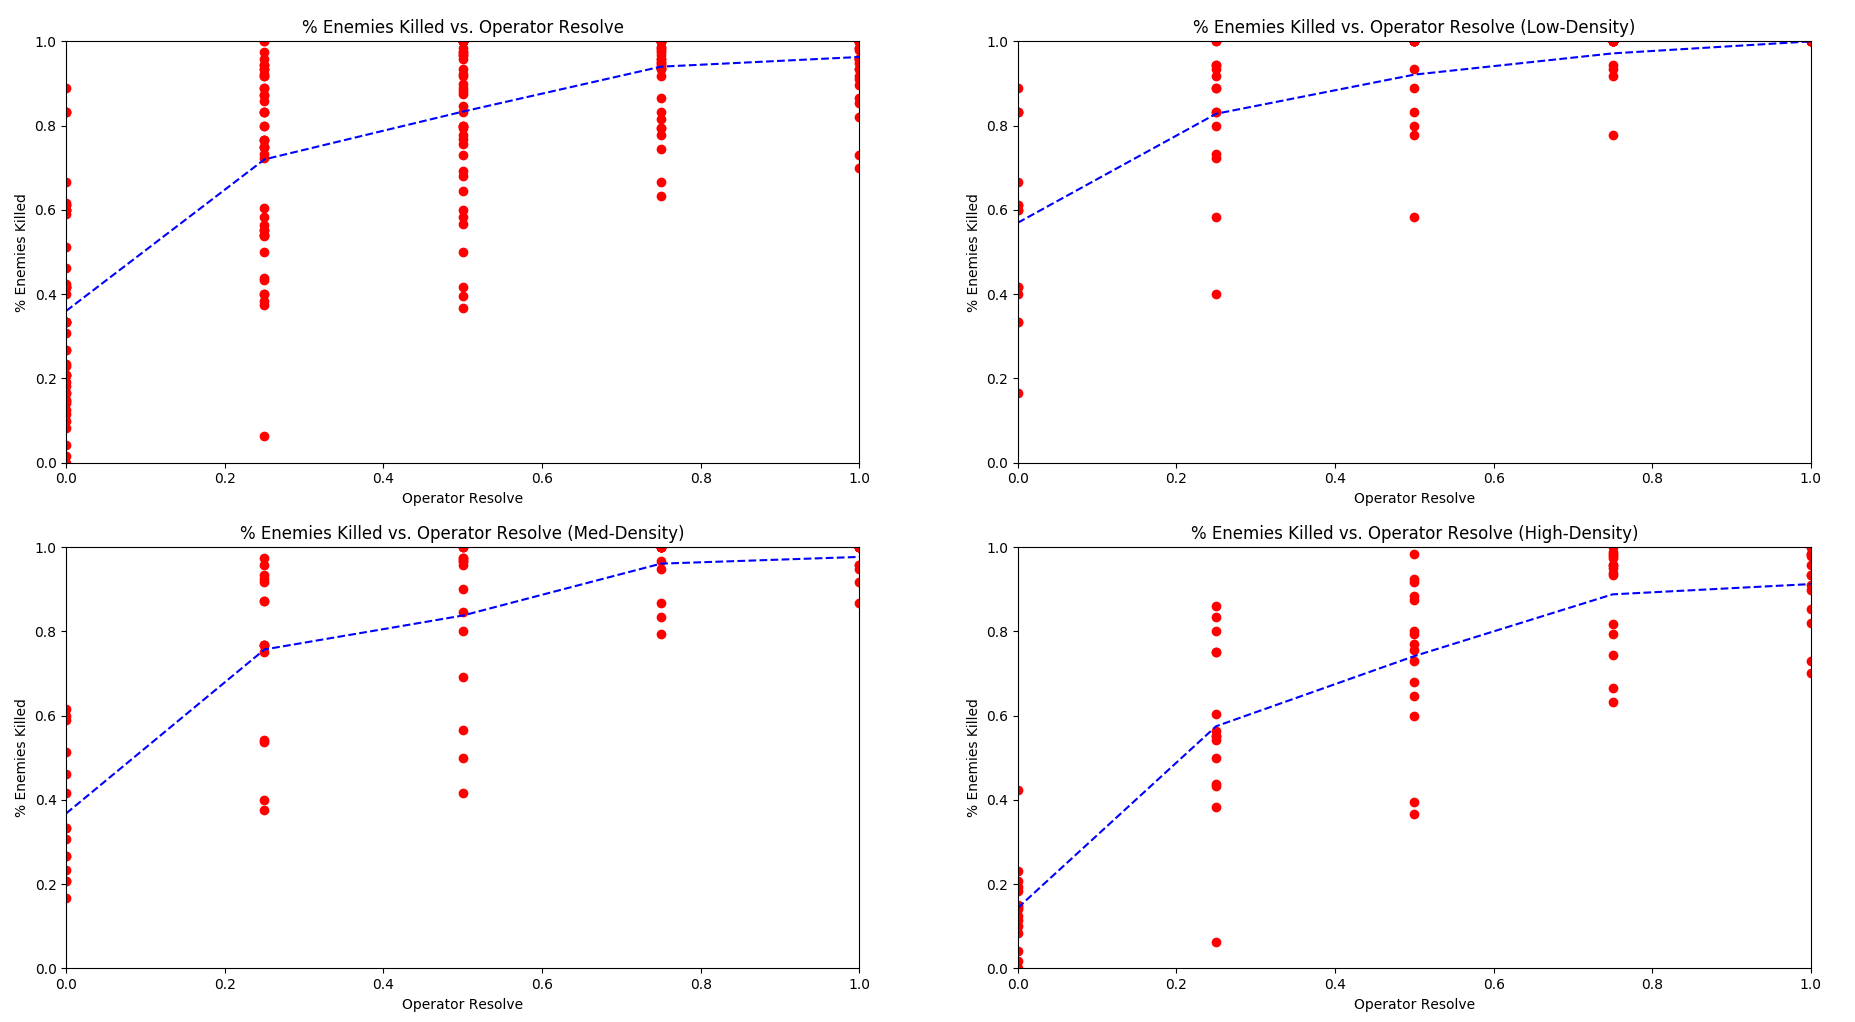
\includegraphics[width=\linewidth]{figures/ScatPlotsOptrsEnemies}
			\subcaption{Scatterplots of enemy death rates compared to operator resolve.}
			\label{fig:ScatPlotsOptrsEnemies}
		\end{subfigure}
		\begin{subfigure}[b]{\textwidth}
			\centering
			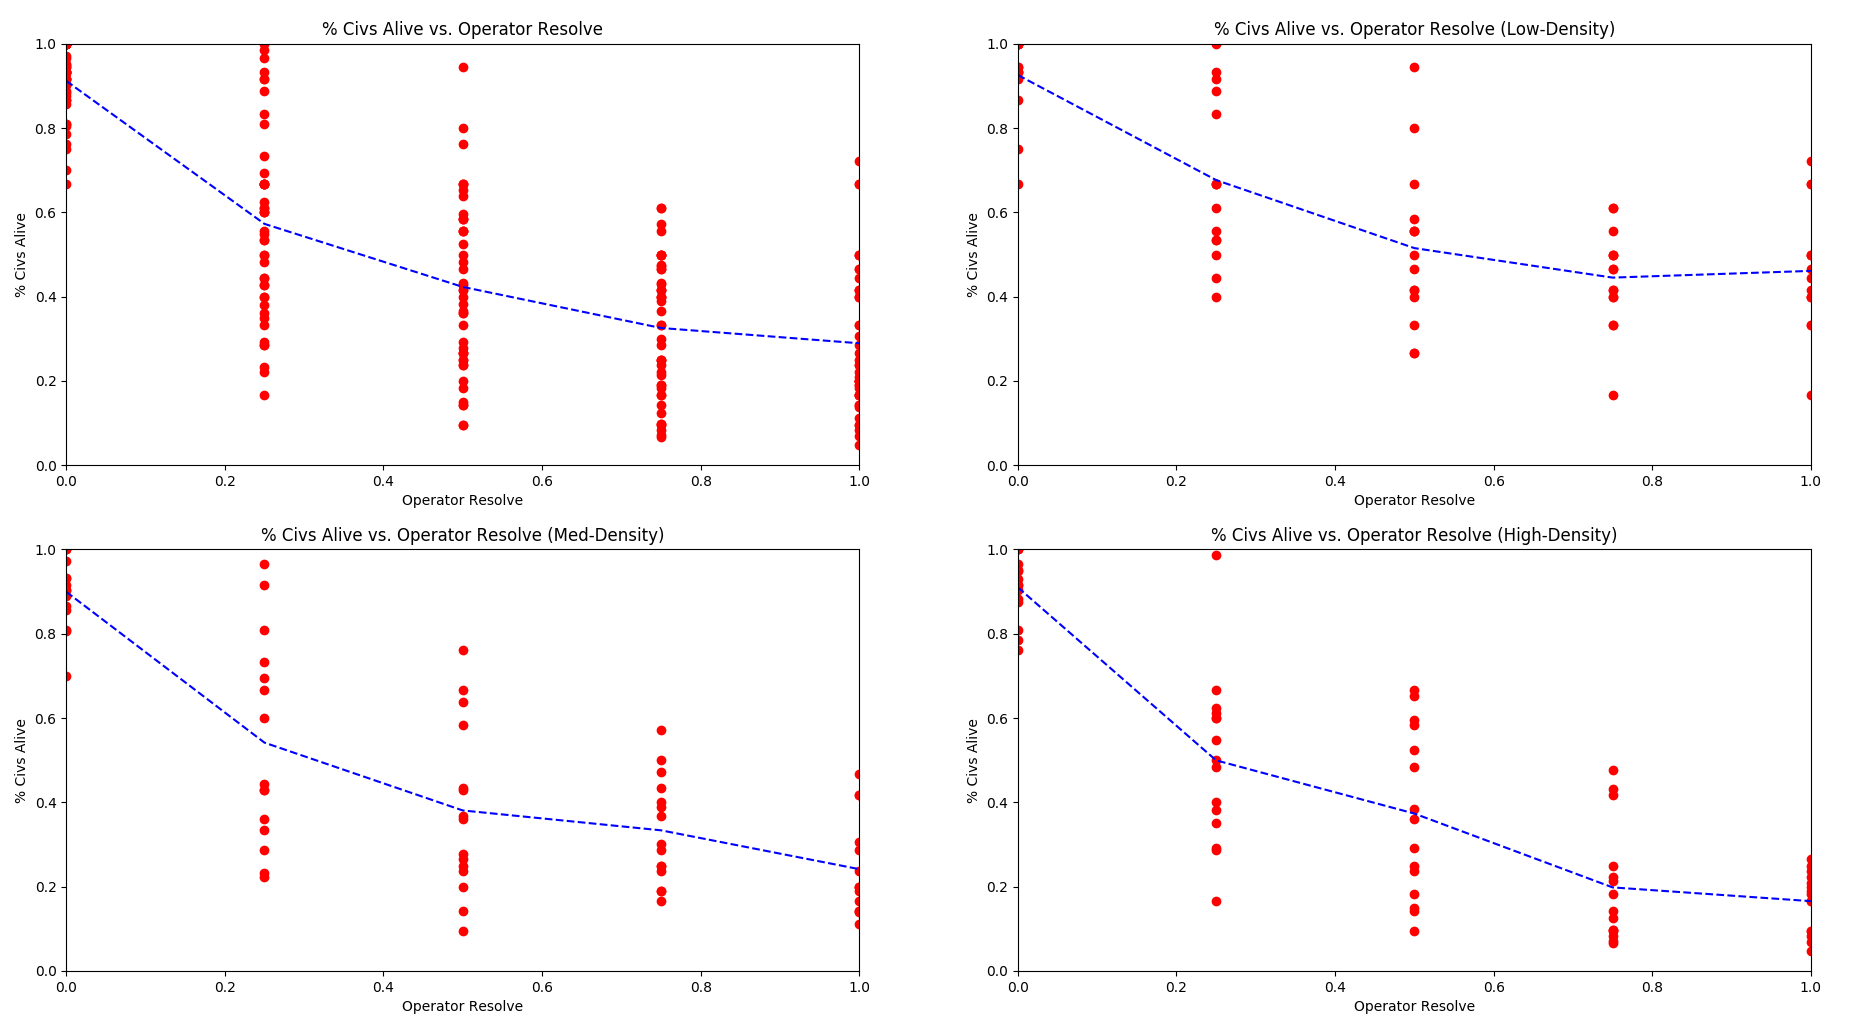
\includegraphics[width=\linewidth]{figures/ScatPlotsOptrsCivs}
			\subcaption{Scatterplots of civilian survival rates compared to operator resolve.}
			\label{fig:ScatPlotsOptrsCivs}
		\end{subfigure}
		\caption{Scatterplots are given for all test (top-left), low-density tests (top-right), medium-density tests (bottom-left), and high-density tests (bottom-right). The dashed blue lines indicate the change in the average proportion for each value.}
		\label{fig:ScatPlotsOptrs}
	\end{figure}

	%% Bibliography stuff
	\pagebreak
	\bibliographystyle{plain}
	\bibliography{cited}
\end{document}